\chapter{Experimental Measurement Results}
\label{ch:measurements}

\section{Overview}
\label{sec:meas_overview}

This chapter presents the results of applying the measurement setup and current-sensing chain of Chapter \ref{ch:measurement_setup} to the physical prototype, following the same experimental structure used for the Simulink simulations of Chapter \ref{ch:simulations}: for each rectifier configuration, the compensation capacitor $C_m$ and the load resistance $R_L$ are first swept independently at $100\ \text{rpm}$, the speed that sets the lower bound on the power available across the target range, before sweeping the resulting configuration across the whole $100$--$400\ \text{rpm}$ range and evaluating its rectifier efficiency. Unlike those simulations, which swept $C_m$ at both ends of the target speed range to identify the two limiting values used in the frequency sweep, the compensation capacitor of the prototype was swept only at $100\ \text{rpm}$; the smaller value needed at the top of the range is instead identified directly within the frequency sweep itself, by comparing several fixed values of $C_m$ across the whole range, as described below. As in Chapter \ref{ch:simulations}, the filter capacitor is fixed at $C_r=1480\ \mu\text{F}$ throughout this chapter.

Where the prototype allows it, the bridges of a configuration are measured not only individually, each loaded by its own resistor, but also already wired together in parallel onto a single shared load, giving a genuinely combined measurement rather than the sum of two or three independent ones. Both the individual and the combined figures are shown wherever available.

\section{Full-Wave Rectifier (FWR)}
\label{sec:meas_fwr}

\subsection{Star Connection}
\label{sec:meas_fwr_star}

\subsubsection{Compensation Capacitor ($C_m$) Sweep}

With the load fixed at $R_L=11\ \Omega$, $C_m$ was swept at $100\ \text{rpm}$ for both bridges of the star connection. Figure \ref{fig:meas_fwr_star_cm} shows the output power of FWR1 rising from $17.22\ \text{mW}$ at $C_m=330\ \mu\text{F}$ to a broad maximum extending from about $530$ to $730\ \mu\text{F}$, peaking at $20.03\ \text{mW}$ at $C_m=630\ \mu\text{F}$. FWR2 follows a similar shape but peaks later, at $C_m=730\ \mu\text{F}$ ($20.74\ \text{mW}$), with its own plateau extending from about $630$ to $830\ \mu\text{F}$; below $C_m=530\ \mu\text{F}$, FWR2 delivers noticeably less power than FWR1, the reverse of the ordering seen near the two bridges' peaks. The combined power of the two bridges peaks at $C_m=730\ \mu\text{F}$ ($40.68\ \text{mW}$), only about $1\%$ above its value at $C_m=630\ \mu\text{F}$ ($40.31\ \text{mW}$); given how flat the combined curve is across this range, $C_m=630\ \mu\text{F}$ was chosen and carried forward to the load resistance sweep below.

\begin{figure}[h!]
    \centering
    
\includegraphics[width=0.7\textwidth]{Measure/Y/Cs_comp.pdf}
    \caption{Output power of the star-connected first and second bridges as a function of the compensation capacitor $C_m$, measured at $100\ \text{rpm}$ ($C_r=1480\ \mu\text{F}$, $R_L=11\ \Omega$).}
    \label{fig:meas_fwr_star_cm}
\end{figure}

\subsubsection{Load Resistance ($R_L$) Sweep}

With $C_m=630\ \mu\text{F}$ fixed, the load resistance of each bridge was swept individually at $100\ \text{rpm}$. Figure \ref{fig:meas_fwr_star_rl} shows both bridges peaking at $R_L=16\ \Omega$ ($21.24\ \text{mW}$ for FWR1, $21.78\ \text{mW}$ for FWR2), with a broad plateau extending from about $13$ to $17$--$19\ \Omega$ depending on the bridge; $R_L=16\ \Omega$ was chosen for each individually-loaded bridge, and is the value used in the frequency sweep and efficiency evaluation below.

The two bridges were then connected together onto a single shared load and swept again, over the narrower range expected for two similar loads in parallel. Figure \ref{fig:meas_fwr_star_rl_tot} shows this combined measurement peaking at $R_L=7\ \Omega$ ($48.36\ \text{mW}$), close to half the $16\ \Omega$ found for each bridge individually, with a plateau again extending from about $5$ to $8\ \Omega$. $R_L=7\ \Omega$ is the value used whenever the two bridges are measured already connected in parallel, in the frequency sweep below.

\begin{figure}[h!]
    \centering
    
\includegraphics[width=0.7\textwidth]{Measure/Y/Rs_comp.pdf}
    \caption{Output power of the star-connected first and second bridges, each individually loaded, as a function of its own load resistance $R_L$, measured at $100\ \text{rpm}$ ($C_r=1480\ \mu\text{F}$, $C_m=630\ \mu\text{F}$).}
    \label{fig:meas_fwr_star_rl}
\end{figure}

\begin{figure}[h!]
    \centering
    
\includegraphics[width=0.7\textwidth]{Measure/Y/Rs_tot.pdf}
    \caption{Output power of the star-connected first and second bridges, already connected in parallel onto a single shared load, as a function of that load resistance $R_L$, measured at $100\ \text{rpm}$ ($C_r=1480\ \mu\text{F}$, $C_m=630\ \mu\text{F}$).}
    \label{fig:meas_fwr_star_rl_tot}
\end{figure}

\subsubsection{Frequency Sweep}

Figures \ref{fig:meas_fwr_star_freq_1} and \ref{fig:meas_fwr_star_freq_2} sweep seven fixed values of $C_m$, from $630\ \mu\text{F}$ down to $47\ \mu\text{F}$, across the whole target speed range, with $R_L=16\ \Omega$ fixed for each individually-loaded bridge. At $100\ \text{rpm}$, $C_m=630\ \mu\text{F}$ delivers the most power for both bridges, consistent with the compensation capacitor sweep above, while $C_m=47\ \mu\text{F}$ performs the worst. As speed increases, the best-performing value drops in stages rather than through a single crossover: for FWR1, the lead passes from $C_m=630\ \mu\text{F}$ at $100\ \text{rpm}$, to $330\ \mu\text{F}$ at $150\ \text{rpm}$, to $200\ \mu\text{F}$ at $200\ \text{rpm}$, to $100\ \mu\text{F}$ between $250$ and $300\ \text{rpm}$, and finally to $47\ \mu\text{F}$ at $350$ and $400\ \text{rpm}$, reaching $292.5\ \text{mW}$ at the top of the range. FWR2 follows a similar progression, handing the lead from $630\ \mu\text{F}$ to $430\ \mu\text{F}$ ($150\ \text{rpm}$), $330\ \mu\text{F}$ ($200\ \text{rpm}$), $100\ \mu\text{F}$ ($250$--$350\ \text{rpm}$) and finally $47\ \mu\text{F}$ at $400\ \text{rpm}$, reaching $327.6\ \text{mW}$. As in the simulations of Section \ref{sec:sim_fwr_star}, no single value of $C_m$ is therefore best across the whole range: the small value needed at high speed, identified here from this progression rather than from a dedicated $400\ \text{rpm}$ sweep, plays the same role as the value found in simulation.

\begin{figure}[h!]
    \centering
    
\includegraphics[width=0.7\textwidth]{Measure/Y/Fs_1.pdf}
    \caption{Output power of the first bridge (FWR1) of the star connection across the target speed range, for seven fixed values of the compensation capacitor $C_m$ ($C_r=1480\ \mu\text{F}$, $R_L=16\ \Omega$).}
    \label{fig:meas_fwr_star_freq_1}
\end{figure}

\begin{figure}[h!]
    \centering
    
\includegraphics[width=0.7\textwidth]{Measure/Y/Fs_2.pdf}
    \caption{Output power of the second bridge (FWR2) of the star connection across the target speed range, for seven fixed values of the compensation capacitor $C_m$ ($C_r=1480\ \mu\text{F}$, $R_L=16\ \Omega$).}
    \label{fig:meas_fwr_star_freq_2}
\end{figure}

With the two bridges already connected in parallel onto the shared $R_L=7\ \Omega$ load found above, only the two extreme values of $C_m$ were remeasured across the speed range. Figure \ref{fig:meas_fwr_star_freq_tot} confirms the same crossover already seen individually: $C_m=630\ \mu\text{F}$ delivers more power than $C_m=47\ \mu\text{F}$ from $100$ to $250\ \text{rpm}$ ($47.6$ against $8.7\ \text{mW}$ at $100\ \text{rpm}$, closing to $245.1$ against $199.6\ \text{mW}$ at $250\ \text{rpm}$), after which $C_m=47\ \mu\text{F}$ takes over and pulls ahead for the rest of the range, reaching $677.2\ \text{mW}$ against $433.3\ \text{mW}$ at $400\ \text{rpm}$.

\begin{figure}[h!]
    \centering
    
\includegraphics[width=0.7\textwidth]{Measure/Y/Fs_tot.pdf}
    \caption{Combined output power of the star-connected bridges, already connected in parallel, across the target speed range, for the two extreme values of the compensation capacitor $C_m$ ($C_r=1480\ \mu\text{F}$, $R_L=7\ \Omega$).}
    \label{fig:meas_fwr_star_freq_tot}
\end{figure}

\subsubsection{Efficiency}

Figures \ref{fig:meas_fwr_star_eff_1} and \ref{fig:meas_fwr_star_eff_2} show the rectifier efficiency $\eta_\text{Rec}=P_\text{out}/P_\text{in}$ of each individually-loaded bridge, for the same seven values of $C_m$, across the speed range. As in the simulations, no DC-DC converter stage is included here, so $\eta_\text{Rec}$ coincides with the full PCE of \eqref{eq:pce} once such a stage is added. Both bridges show the same qualitative behaviour: $\eta_\text{Rec}$ is lowest for the smallest capacitor and highest for the largest one at $100\ \text{rpm}$, ranging from $0.275$ to $0.408$ for FWR1 and from $0.235$ to $0.413$ for FWR2; the seven curves then converge by $400\ \text{rpm}$ to a narrow band, $0.548$--$0.567$ for FWR1 and $0.52$--$0.57$ for FWR2. The measured values at $100\ \text{rpm}$ sit close to the $\eta_\text{Rec}\approx0.20$--$0.43$ found in simulation (Section \ref{sec:sim_fwr_star}), but the values measured at $400\ \text{rpm}$ are noticeably lower than the simulated $\eta_\text{Rec}\approx0.70$--$0.76$.

\begin{figure}[h!]
    \centering
    
\includegraphics[width=0.65\textwidth]{Measure/Y/Eff_1.pdf}
    \caption{Rectifier efficiency $\eta_\text{Rec}$ of the first bridge (FWR1) of the star connection across the target speed range, for seven fixed values of the compensation capacitor $C_m$ ($C_r=1480\ \mu\text{F}$, $R_L=16\ \Omega$).}
    \label{fig:meas_fwr_star_eff_1}
\end{figure}

\begin{figure}[h!]
    \centering
    
\includegraphics[width=0.65\textwidth]{Measure/Y/Eff_2.pdf}
    \caption{Rectifier efficiency $\eta_\text{Rec}$ of the second bridge (FWR2) of the star connection across the target speed range, for seven fixed values of the compensation capacitor $C_m$ ($C_r=1480\ \mu\text{F}$, $R_L=16\ \Omega$).}
    \label{fig:meas_fwr_star_eff_2}
\end{figure}

\clearpage
\subsection{Delta Connection}
\label{sec:meas_fwr_delta}

\subsubsection{Compensation Capacitor ($C_m$) Sweep}

With $R_L=5\ \Omega$ fixed, $C_m$ was swept at $100\ \text{rpm}$ for both bridges of the delta connection. Figure \ref{fig:meas_fwr_delta_cm} shows FWR1 peaking at $C_m=630\ \mu\text{F}$ ($8.92\ \text{mW}$), with a plateau extending from about $530$ to $630\ \mu\text{F}$, and FWR2 peaking at the same value ($7.97\ \text{mW}$), with its own plateau extending slightly further, to about $730\ \mu\text{F}$. Unlike the star connection, both bridges share the same peak location here, and the combined power peaks sharply at $C_m=630\ \mu\text{F}$ ($16.89\ \text{mW}$), which was chosen and carried forward to the load resistance sweep below.

\begin{figure}[h!]
    \centering
    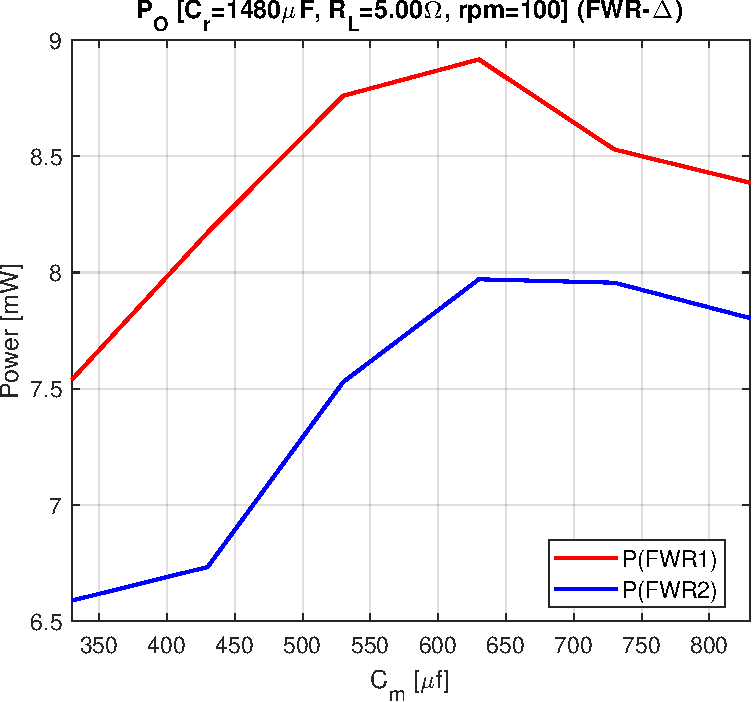
\includegraphics[width=0.7\textwidth]{Measure/D/Cs_comp.pdf}
    \caption{Output power of the delta-connected first and second bridges as a function of the compensation capacitor $C_m$, measured at $100\ \text{rpm}$ ($C_r=1480\ \mu\text{F}$, $R_L=5\ \Omega$).}
    \label{fig:meas_fwr_delta_cm}
\end{figure}

\subsubsection{Load Resistance ($R_L$) Sweep}

With $C_m=630\ \mu\text{F}$ fixed, the load resistance of each bridge was swept individually at $100\ \text{rpm}$. Figure \ref{fig:meas_fwr_delta_rl} shows both bridges peaking at $R_L=7\ \Omega$ ($9.14\ \text{mW}$ for FWR1, $7.97\ \text{mW}$ for FWR2), with a broad plateau extending from about $6$ to $8$--$9\ \Omega$; $R_L=7\ \Omega$ was chosen for each individually-loaded bridge.

The two bridges were then connected together onto a single shared load. Figure \ref{fig:meas_fwr_delta_rl_tot} shows this combined measurement peaking at $R_L=4\ \Omega$ ($14.48\ \text{mW}$), close to half the $7\ \Omega$ found for each bridge individually, with a plateau extending from about $3$ to $5\ \Omega$; $R_L=5\ \Omega$, within this plateau, is the value used whenever the two bridges are measured already connected in parallel, in the frequency sweep below.

\begin{figure}[h!]
    \centering
    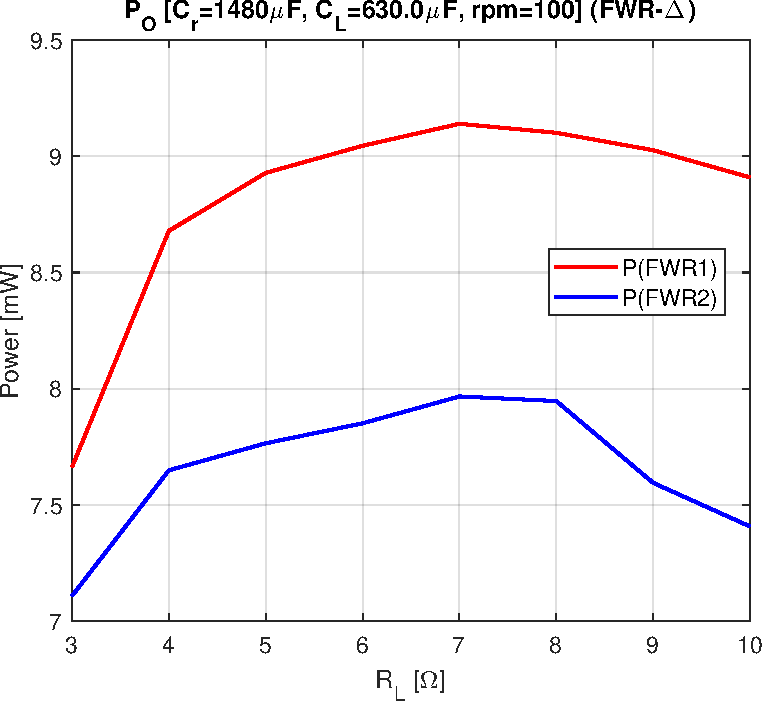
\includegraphics[width=0.7\textwidth]{Measure/D/Rs_comp.pdf}
    \caption{Output power of the delta-connected first and second bridges, each individually loaded, as a function of its own load resistance $R_L$, measured at $100\ \text{rpm}$ ($C_r=1480\ \mu\text{F}$, $C_m=630\ \mu\text{F}$).}
    \label{fig:meas_fwr_delta_rl}
\end{figure}

\begin{figure}[h!]
    \centering
    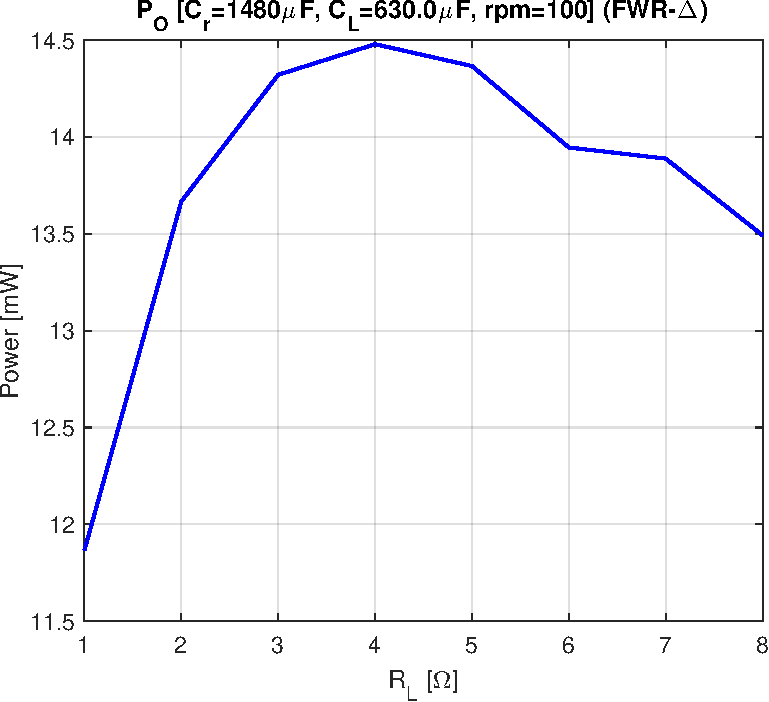
\includegraphics[width=0.7\textwidth]{Measure/D/Rs_tot.pdf}
    \caption{Output power of the delta-connected first and second bridges, already connected in parallel onto a single shared load, as a function of that load resistance $R_L$, measured at $100\ \text{rpm}$ ($C_r=1480\ \mu\text{F}$, $C_m=630\ \mu\text{F}$).}
    \label{fig:meas_fwr_delta_rl_tot}
\end{figure}

\subsubsection{Frequency Sweep}

Figures \ref{fig:meas_fwr_delta_freq_1} and \ref{fig:meas_fwr_delta_freq_2} sweep the same seven fixed values of $C_m$ across the whole target speed range, with $R_L=7\ \Omega$ fixed for each individually-loaded bridge. FWR1 hands the lead from $C_m=630\ \mu\text{F}$ at $100$--$150\ \text{rpm}$, to $430\ \mu\text{F}$ at $200\ \text{rpm}$, to $200\ \mu\text{F}$ from $250$ to $350\ \text{rpm}$, and finally to $47\ \mu\text{F}$ at $400\ \text{rpm}$, reaching $201.3\ \text{mW}$. FWR2 follows a simpler, single handoff: $C_m=630\ \mu\text{F}$ leads until $150\ \text{rpm}$, after which $C_m=330\ \mu\text{F}$ takes over for the rest of the range, reaching $196.1\ \text{mW}$ at $400\ \text{rpm}$.

\begin{figure}[h!]
    \centering
    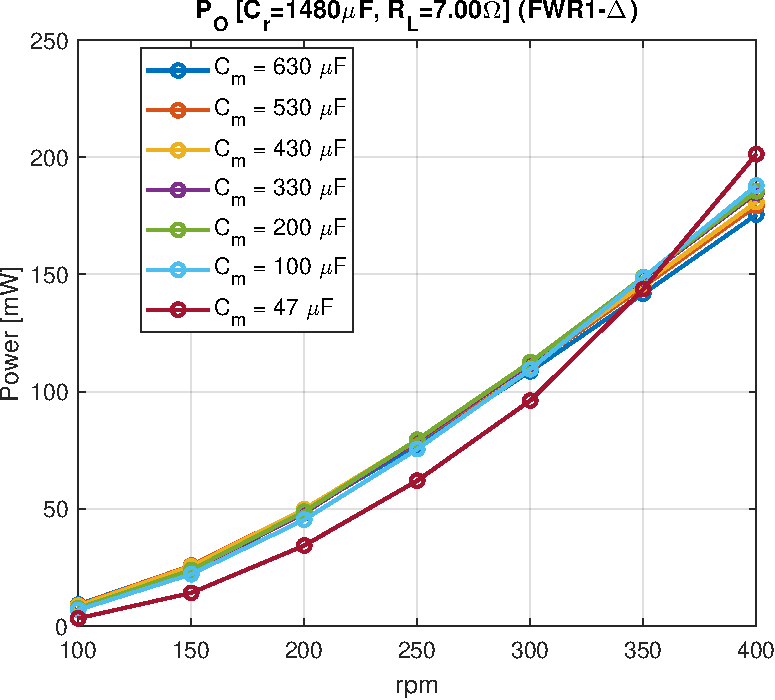
\includegraphics[width=0.7\textwidth]{Measure/D/Fs_1.pdf}
    \caption{Output power of the first bridge (FWR1) of the delta connection across the target speed range, for seven fixed values of the compensation capacitor $C_m$ ($C_r=1480\ \mu\text{F}$, $R_L=7\ \Omega$).}
    \label{fig:meas_fwr_delta_freq_1}
\end{figure}

\begin{figure}[h!]
    \centering
    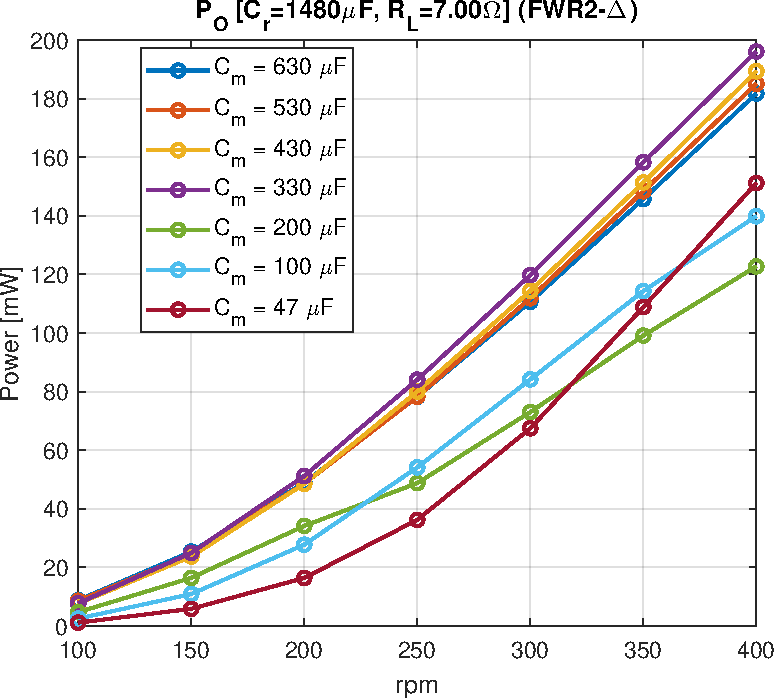
\includegraphics[width=0.7\textwidth]{Measure/D/Fs_2.pdf}
    \caption{Output power of the second bridge (FWR2) of the delta connection across the target speed range, for seven fixed values of the compensation capacitor $C_m$ ($C_r=1480\ \mu\text{F}$, $R_L=7\ \Omega$).}
    \label{fig:meas_fwr_delta_freq_2}
\end{figure}

With the two bridges already connected in parallel onto the shared $R_L=5\ \Omega$ load, Figure \ref{fig:meas_fwr_delta_freq_tot} again compares only the two extreme values of $C_m$: $C_m=630\ \mu\text{F}$ leads from $100$ to $250\ \text{rpm}$ ($14.9$ against $6.5\ \text{mW}$ at $100\ \text{rpm}$, closing to $133.9$ against $123.6\ \text{mW}$ at $250\ \text{rpm}$), after which $C_m=47\ \mu\text{F}$ overtakes it and pulls ahead, reaching $368.2\ \text{mW}$ against $310.7\ \text{mW}$ at $400\ \text{rpm}$, the same crossover speed already seen for the star connection.

\begin{figure}[h!]
    \centering
    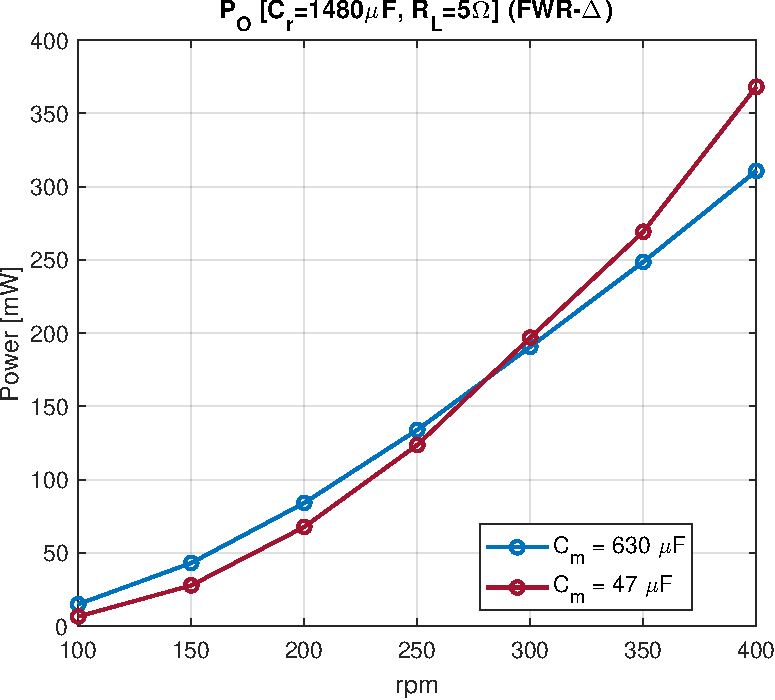
\includegraphics[width=0.7\textwidth]{Measure/D/Fs_tot.pdf}
    \caption{Combined output power of the delta-connected bridges, already connected in parallel, across the target speed range, for the two extreme values of the compensation capacitor $C_m$ ($C_r=1480\ \mu\text{F}$, $R_L=5\ \Omega$).}
    \label{fig:meas_fwr_delta_freq_tot}
\end{figure}

\subsubsection{Efficiency}

Figures \ref{fig:meas_fwr_delta_eff_1} and \ref{fig:meas_fwr_delta_eff_2} show the rectifier efficiency of each individually-loaded bridge for the same seven values of $C_m$. At $100\ \text{rpm}$, $\eta_\text{Rec}$ ranges from $0.182$ to $0.301$ for FWR1 and from $0.157$ to $0.315$ for FWR2; both ranges converge by $400\ \text{rpm}$ to a narrow band, $0.484$--$0.509$ for FWR1 and $0.482$--$0.512$ for FWR2. These values are lower than the star connection's at both ends of the range ($0.235$--$0.413$ at $100\ \text{rpm}$, $0.52$--$0.57$ at $400\ \text{rpm}$), consistent with Section \ref{sec:fwr}: without the star connection's $\sqrt{3}$ voltage gain, the fixed two-diode-drop loss of the FWR removes a larger fraction of the lower delta line voltage.

\begin{figure}[h!]
    \centering
    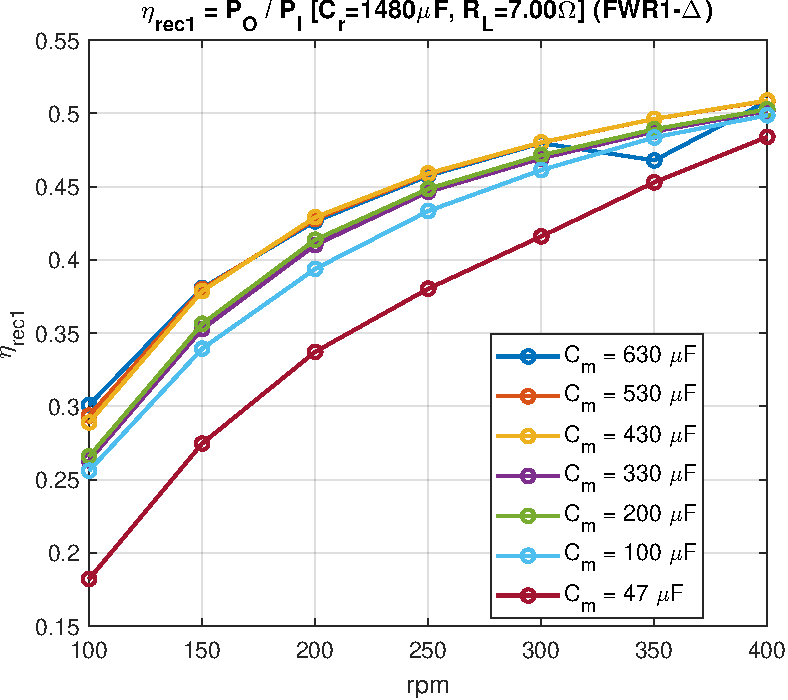
\includegraphics[width=0.65\textwidth]{Measure/D/Eff_1.pdf}
    \caption{Rectifier efficiency $\eta_\text{Rec}$ of the first bridge (FWR1) of the delta connection across the target speed range, for seven fixed values of the compensation capacitor $C_m$ ($C_r=1480\ \mu\text{F}$, $R_L=7\ \Omega$).}
    \label{fig:meas_fwr_delta_eff_1}
\end{figure}

\begin{figure}[h!]
    \centering
    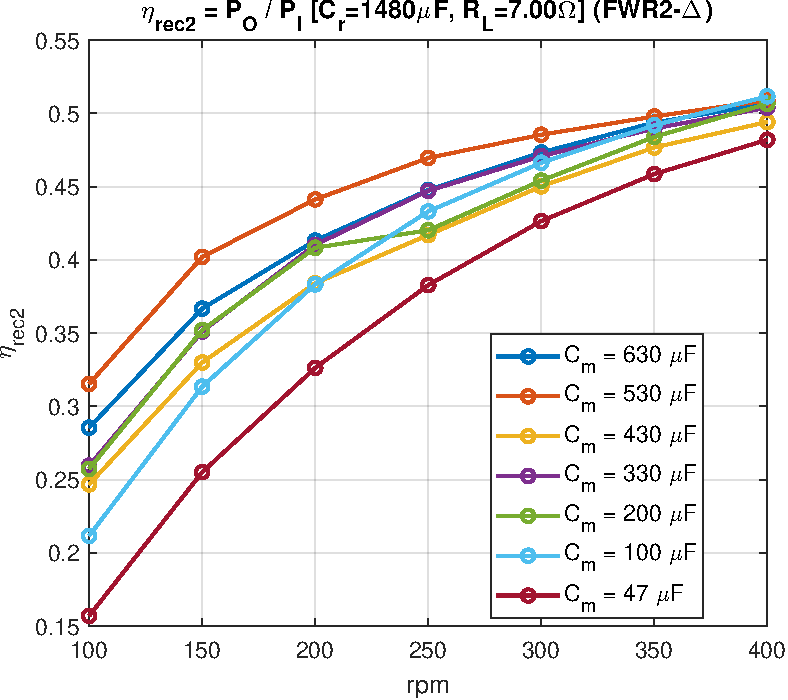
\includegraphics[width=0.65\textwidth]{Measure/D/Eff_2.pdf}
    \caption{Rectifier efficiency $\eta_\text{Rec}$ of the second bridge (FWR2) of the delta connection across the target speed range, for seven fixed values of the compensation capacitor $C_m$ ($C_r=1480\ \mu\text{F}$, $R_L=7\ \Omega$).}
    \label{fig:meas_fwr_delta_eff_2}
\end{figure}

\clearpage
\section{Negative Voltage Converter (NVC)}
\label{sec:meas_nvc}

\subsection{Compensation Capacitor ($C_m$) Sweep}
\label{sec:meas_nvc_cm}

With $R_L=20\ \Omega$ fixed for each of the three bridges, $C_m$ was swept at $100\ \text{rpm}$. Figure \ref{fig:meas_nvc_cm} shows all three bridges rising steeply for small $C_m$ and peaking together around $C_m=430\ \mu\text{F}$: NVC1 reaches $21.88\ \text{mW}$, NVC2 $20.80\ \text{mW}$, and NVC3, delivering noticeably less than the other two, $17.96\ \text{mW}$, about $18\%$ less than NVC1 and $14\%$ less than NVC2 at the peak, closely matching the gap already seen in simulation (Section \ref{sec:sim_nvc_cm}). All three bridges then decrease only very gently for larger $C_m$, NVC3 in particular staying within a few percent of its peak all the way to $C_m=830\ \mu\text{F}$. The combined power of the three bridges peaks at the same value, $C_m=430\ \mu\text{F}$ ($60.65\ \text{mW}$), which was chosen and carried forward to the load resistance sweep below.

\begin{figure}[h!]
    \centering
    
\includegraphics[width=0.7\textwidth]{Measure/NVC/Cs_comp.pdf}
    \caption{Output power of the three NVC bridges as a function of the compensation capacitor $C_m$, measured at $100\ \text{rpm}$ ($C_r=1480\ \mu\text{F}$, $R_L=20\ \Omega$).}
    \label{fig:meas_nvc_cm}
\end{figure}

\subsection{Load Resistance ($R_L$) Sweep}
\label{sec:meas_nvc_rl}

With $C_m=430\ \mu\text{F}$ fixed, the load resistance of each bridge was swept individually at $100\ \text{rpm}$. Figure \ref{fig:meas_nvc_rl} shows all three bridges peaking within a few ohms of each other, NVC1 at $R_L=25\ \Omega$ ($21.86\ \text{mW}$), NVC2 and NVC3 both at $R_L=21\ \Omega$ ($20.71\ \text{mW}$ and $17.30\ \text{mW}$ respectively), with every bridge staying within about $2\%$ of its own peak across a broad range from about $18$ to $27$--$28\ \Omega$. Summing the three individually-loaded bridges, Figure \ref{fig:meas_nvc_rl_tot} shows the combined power peaking at $R_L=21\ \Omega$ ($59.62\ \text{mW}$) and staying close to this maximum across almost the whole range swept. $R_L=21\ \Omega$ was chosen for NVC2 and NVC3, and $R_L=24\ \Omega$, still well within the broad plateau, for NVC1; these are the values used in the frequency sweep below.

\begin{figure}[h!]
    \centering
    
\includegraphics[width=0.7\textwidth]{Measure/NVC/Rs_comp.pdf}
    \caption{Output power of the three NVC bridges, each individually loaded, as a function of its own load resistance $R_L$, measured at $100\ \text{rpm}$ ($C_r=1480\ \mu\text{F}$, $C_m=430\ \mu\text{F}$).}
    \label{fig:meas_nvc_rl}
\end{figure}

\begin{figure}[h!]
    \centering
    
\includegraphics[width=0.7\textwidth]{Measure/NVC/Rs_tot.pdf}
    \caption{Combined output power of the three individually-loaded NVC bridges, obtained by summing the three curves of Figure \ref{fig:meas_nvc_rl}, as a function of their common load resistance $R_L$, measured at $100\ \text{rpm}$ ($C_r=1480\ \mu\text{F}$, $C_m=430\ \mu\text{F}$).}
    \label{fig:meas_nvc_rl_tot}
\end{figure}

\subsection{Frequency Sweep}
\label{sec:meas_nvc_freq}

Figures \ref{fig:meas_nvc_freq_1}--\ref{fig:meas_nvc_freq_3} sweep five fixed values of $C_m$, from $430\ \mu\text{F}$ down to $47\ \mu\text{F}$, across the whole target speed range, with $R_L=24\ \Omega$, $21\ \Omega$ and $21\ \Omega$ fixed for NVC1, NVC2 and NVC3 respectively. As with the FWR bridges, the best-performing value of $C_m$ shifts in stages as speed increases, rather than through a single crossover. NVC1 and NVC2 follow a similar progression, handing the lead from $C_m=430\ \mu\text{F}$ at $100\ \text{rpm}$, to $200\ \mu\text{F}$ at $150\ \text{rpm}$, to $100\ \mu\text{F}$ at $200\ \text{rpm}$ (NVC2 already reaches $C_m=47\ \mu\text{F}$ by $250\ \text{rpm}$, one step ahead of NVC1, which does so only from $300\ \text{rpm}$), reaching $287.8\ \text{mW}$ and $210.5\ \text{mW}$ respectively at $400\ \text{rpm}$. NVC3 instead settles on $C_m=100\ \mu\text{F}$ from $150\ \text{rpm}$ onward and never hands the lead to $C_m=47\ \mu\text{F}$, reaching $174.0\ \text{mW}$ at $400\ \text{rpm}$ against $151.8\ \text{mW}$ for $C_m=47\ \mu\text{F}$; unlike NVC1 and NVC2, NVC3 shows no clear benefit from the smallest capacitor even at the top of the range.

\begin{figure}[h!]
    \centering
    
\includegraphics[width=0.7\textwidth]{Measure/NVC/Fs_1.pdf}
    \caption{Output power of NVC1 across the target speed range, for five fixed values of the compensation capacitor $C_m$ ($C_r=1480\ \mu\text{F}$, $R_L=24\ \Omega$).}
    \label{fig:meas_nvc_freq_1}
\end{figure}

\begin{figure}[h!]
    \centering
    
\includegraphics[width=0.7\textwidth]{Measure/NVC/Fs_2.pdf}
    \caption{Output power of NVC2 across the target speed range, for five fixed values of the compensation capacitor $C_m$ ($C_r=1480\ \mu\text{F}$, $R_L=21\ \Omega$).}
    \label{fig:meas_nvc_freq_2}
\end{figure}

\begin{figure}[h!]
    \centering
    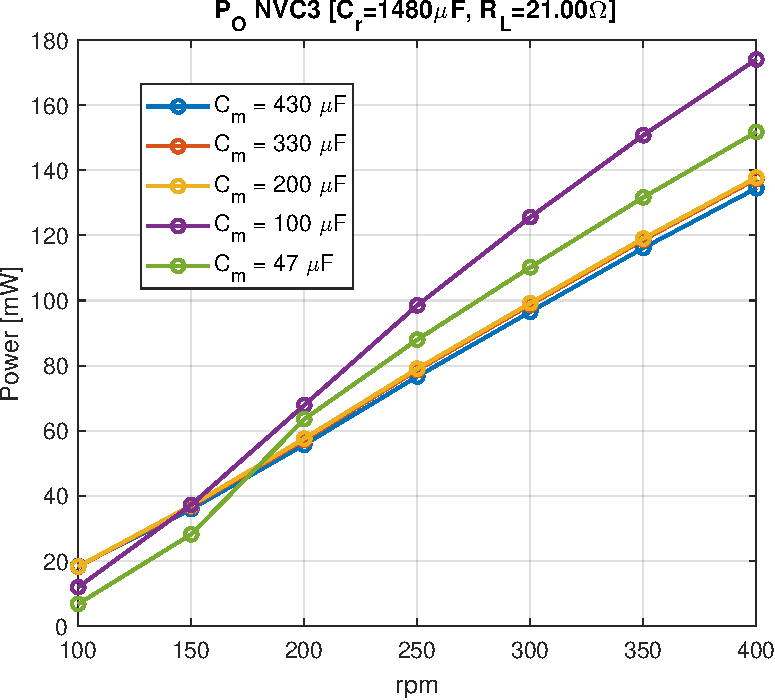
\includegraphics[width=0.7\textwidth]{Measure/NVC/Fs_3.pdf}
    \caption{Output power of NVC3 across the target speed range, for five fixed values of the compensation capacitor $C_m$ ($C_r=1480\ \mu\text{F}$, $R_L=21\ \Omega$).}
    \label{fig:meas_nvc_freq_3}
\end{figure}

With the three bridges already connected in parallel onto a shared $R_L=6\ \Omega$ load, Figure \ref{fig:meas_nvc_freq_tot} shows the same kind of staged hand-off in the combined power: $C_m=430\ \mu\text{F}$ leads at $100\ \text{rpm}$ ($57.7\ \text{mW}$), $C_m=200\ \mu\text{F}$ briefly takes over at $150\ \text{rpm}$ ($121.6\ \text{mW}$), $C_m=100\ \mu\text{F}$ leads from $200$ to $250\ \text{rpm}$ (reaching $302.7\ \text{mW}$, only marginally ahead of $C_m=47\ \mu\text{F}$'s $300.6\ \text{mW}$ by the top of this range), after which $C_m=47\ \mu\text{F}$ takes over for the rest of the range, reaching $603.0\ \text{mW}$ at $400\ \text{rpm}$ against $511.1\ \text{mW}$ for $C_m=100\ \mu\text{F}$. As with the FWR bridges, no single value of $C_m$ is therefore best across the whole range, and $C_m=430\ \mu\text{F}$, the value found optimal at $100\ \text{rpm}$, remains the preferred choice to keep the power available at the low-speed end of the range as high as possible.

\begin{figure}[h!]
    \centering
    
\includegraphics[width=0.7\textwidth]{Measure/NVC/Fs_tot.pdf}
    \caption{Combined output power of the three NVC bridges, already connected in parallel, across the target speed range, for five fixed values of the compensation capacitor $C_m$ ($C_r=1480\ \mu\text{F}$, $R_L=6\ \Omega$).}
    \label{fig:meas_nvc_freq_tot}
\end{figure}

\subsection{Efficiency}
\label{sec:meas_nvc_eff}

Figure \ref{fig:meas_nvc_eff} shows the rectifier efficiency of the three NVC bridges combined, already connected in parallel, for the same five values of $C_m$. At $100\ \text{rpm}$, $\eta_\text{Rec}$ ranges from $0.461$ for the smallest capacitor ($C_m=47\ \mu\text{F}$) to $0.568$ for the largest one ($C_m=430\ \mu\text{F}$); by $400\ \text{rpm}$ the five curves converge to a narrower band, $\eta_\text{Rec}\approx0.663$--$0.701$. As with the FWR bridges, the curves are ordered consistently with $C_m$ at $100\ \text{rpm}$ and converge at high speed; the values measured at $100\ \text{rpm}$ sit close to the $\eta_\text{Rec}\approx0.24$--$0.67$ found in simulation (Section \ref{sec:sim_nvc_eff}), while those measured at $400\ \text{rpm}$ ($0.663$--$0.701$) fall short of the simulated $\eta_\text{Rec}\approx0.76$--$0.83$.

\begin{figure}[h!]
    \centering
    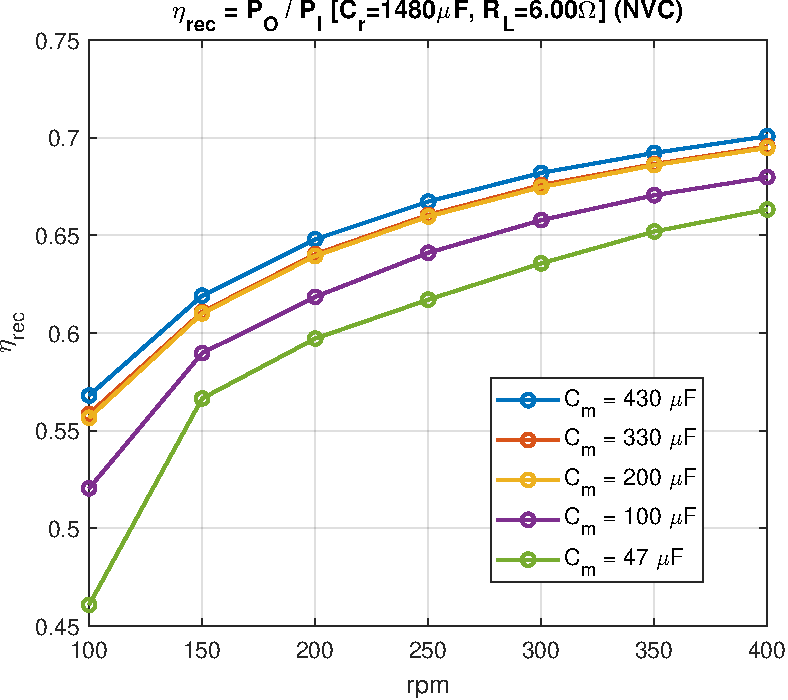
\includegraphics[width=0.65\textwidth]{Measure/NVC/Eff_tot.pdf}
    \caption{Rectifier efficiency $\eta_\text{Rec}$ of the three NVC bridges combined, already connected in parallel, across the target speed range, for five fixed values of the compensation capacitor $C_m$ ($C_r=1480\ \mu\text{F}$, $R_L=6\ \Omega$).}
    \label{fig:meas_nvc_eff}
\end{figure}

\section{Comparison Between Topologies}
\label{sec:meas_comparison}

Sections \ref{sec:meas_fwr} and \ref{sec:meas_nvc} evaluate the FWR (star and delta connections) and the NVC independently, each with its own compensation capacitor and load resistance chosen to maximise the output power at $100\ \text{rpm}$. As in the simulations of Section \ref{sec:sim_comparison}, all three configurations rectify the same six pickup units, only regrouped differently, so their measured output power and efficiency can be compared directly. Table \ref{tab:meas_comparison} summarises the resulting operating points and performance of the three configurations at the two ends of the target speed range. Output power is taken from the bridges already connected in parallel onto a single shared load, the real combined measurement available for all three configurations; rectifier efficiency, for which this real combined measurement does not include the input power needed to compute it for the FWR connections, is instead taken as the ratio of the summed output and input power of the individually-loaded bridges of each configuration.

\begin{table}[htbp]
    \centering
    \begin{tabular}{lccc}
        \toprule
        & FWR (Star) & FWR (Delta) & NVC \\
        \midrule
        $C_m$ at $100\ \text{rpm}$ ($\mu\text{F}$) & 630 & 630 & 430 \\
        $C_m$ at $400\ \text{rpm}$ ($\mu\text{F}$) & 47 & 47 & 47 \\
        $R_L$ ($\Omega$) & 7 & 5 & 6 \\
        $P_O$ at $100\ \text{rpm}$ (mW) & 47.6 & 14.9 & 57.7 \\
        $P_O$ at $400\ \text{rpm}$ (mW) & 433.3 & 310.7 & 425.7 \\
        $\eta_\text{Rec}$ at $100\ \text{rpm}$ & 0.410 & 0.293 & 0.568 \\
        $\eta_\text{Rec}$ at $400\ \text{rpm}$ & 0.564 & 0.508 & 0.701 \\
        \bottomrule
    \end{tabular}
    \caption{Comparison of the three rectifier configurations at their respective chosen operating points, using the $C_m$ found optimal at $100\ \text{rpm}$ for the output power and efficiency figures. $R_L$, and the output power it is measured at, refer to the bridges already connected in parallel onto a shared load; $\eta_\text{Rec}$ is computed from the individually-loaded bridges instead (Sections \ref{sec:meas_fwr_star}--\ref{sec:meas_nvc}).}
    \label{tab:meas_comparison}
\end{table}

At $100\ \text{rpm}$, the NVC delivers the most output power of the three configurations ($57.7\ \text{mW}$), slightly ahead of the star connection ($47.6\ \text{mW}$) and close to four times the delta connection ($14.9\ \text{mW}$). At $400\ \text{rpm}$, the picture is closer than in simulation: the star connection now edges ahead of the NVC ($433.3$ against $425.7\ \text{mW}$, a gap of under $2\%$), while the delta connection remains clearly behind both ($310.7\ \text{mW}$). Between the two FWR connections, the star connection consistently outperforms the delta connection at both speeds, consistent with Section \ref{sec:fwr}: the $\sqrt{3}$ line-to-line voltage gain of the star connection more than compensates for its lower line current, whereas the delta connection's lower line voltage is hit harder by the FWR's fixed two-diode-drop loss.

The rectifier efficiency follows the same ranking as in simulation at both speeds: the NVC leads ($0.568$ at $100\ \text{rpm}$, $0.701$ at $400\ \text{rpm}$), followed by the star connection ($0.410$, $0.564$) and then the delta connection ($0.293$, $0.508$), consistent with the same two-diode-drop mechanism discussed in Section \ref{sec:nvc}: the NVC bridge only replaces the diode drop with the much smaller MOSFET on-resistance once the voltage across its anti-series pair exceeds $V_\text{off}\approx1.2\ \text{V}$, giving it an advantage that persists, if narrower than in simulation, at both ends of the target speed range. Unlike the simulated comparison of Section \ref{sec:sim_comparison}, however, this efficiency advantage no longer translates into the highest output power at the top of the range, where the measured star connection is, within a small margin, the best performer instead. A closer look at how these measured figures relate to the simulations of Chapter \ref{ch:simulations} is given in Chapter \ref{ch:comparison}.
